\section{Results and discussion}
% Structure with subsections
% Use of figures/tables (max. 5)
% General description of the results
\subsection{Differentially Expressed Genes and Network creation}

Under the chosen thresholds discussed in \ref{sec:methods-deg} 908 genes were found to be differentially expressed. Around half of them (495) are upregulated, the remaining 413 are downregulated. STRING was able to query 828 of them; using other ID types did not change this. After querying the additional EDS-related genes the resulting network consists of 847 nodes and 6129 edges.

The position of the known EDS genes in the network is on average more central than expected by chance based on degree, clustering coefficient, betweenness centralitiy and closeness centrality. This supports the close relationship between hEDS and other EDS types.

\subsection{Enrichment analysis and clustering}

\begin{itemize}
	\item Cellular Component: Nuclosome, collagen-containing extracellular matrix, chromatin, chromosamal region [TODO: dot plot or graph?]
	\item Biological Progress: nucleosome assembly \& organization, protein-DNA assembly \& organization, cell clycle signaling, regulation \& transition, chromosome separation regulation
	\item Molecular function difficult to analyse on large graph, but we see structural constituent of chromatin, protein heterodimerization activity and extracellular matrix structural constituent
\end{itemize}


TODO

\subsubsection{MCODE}
Running MCODE on the created networks finds 3 clusters with more than 15 nodes, one with 66 nodes and 1953 connections, one with 44 nodes and 686 connections and one with 16 nodes and 114 connections with the second two clusters containing apregulated genes only.

The third, smaller cluster, shown in \ref{fig:mcode3}, contains mostly upregulated but also two downregulated genes. Some do not show a strong differential expression but are genes known to cause other EDS types. In total, the cluster contains eight EDS genes, all having a $|\text{log2FoldChange}| < 0.5$ and nine differentially expressed genes. One of the EDS genes is also one of the two down-regulated genes. All known EDS genes besides ADAMTS2 have a high Closeness Centrality, consistent with the findings of EDS genes being more central in the complete network.

\begin{figure}[htb!]
	\centering
	\caption*{\textbf{MCODE cluster 3}}
	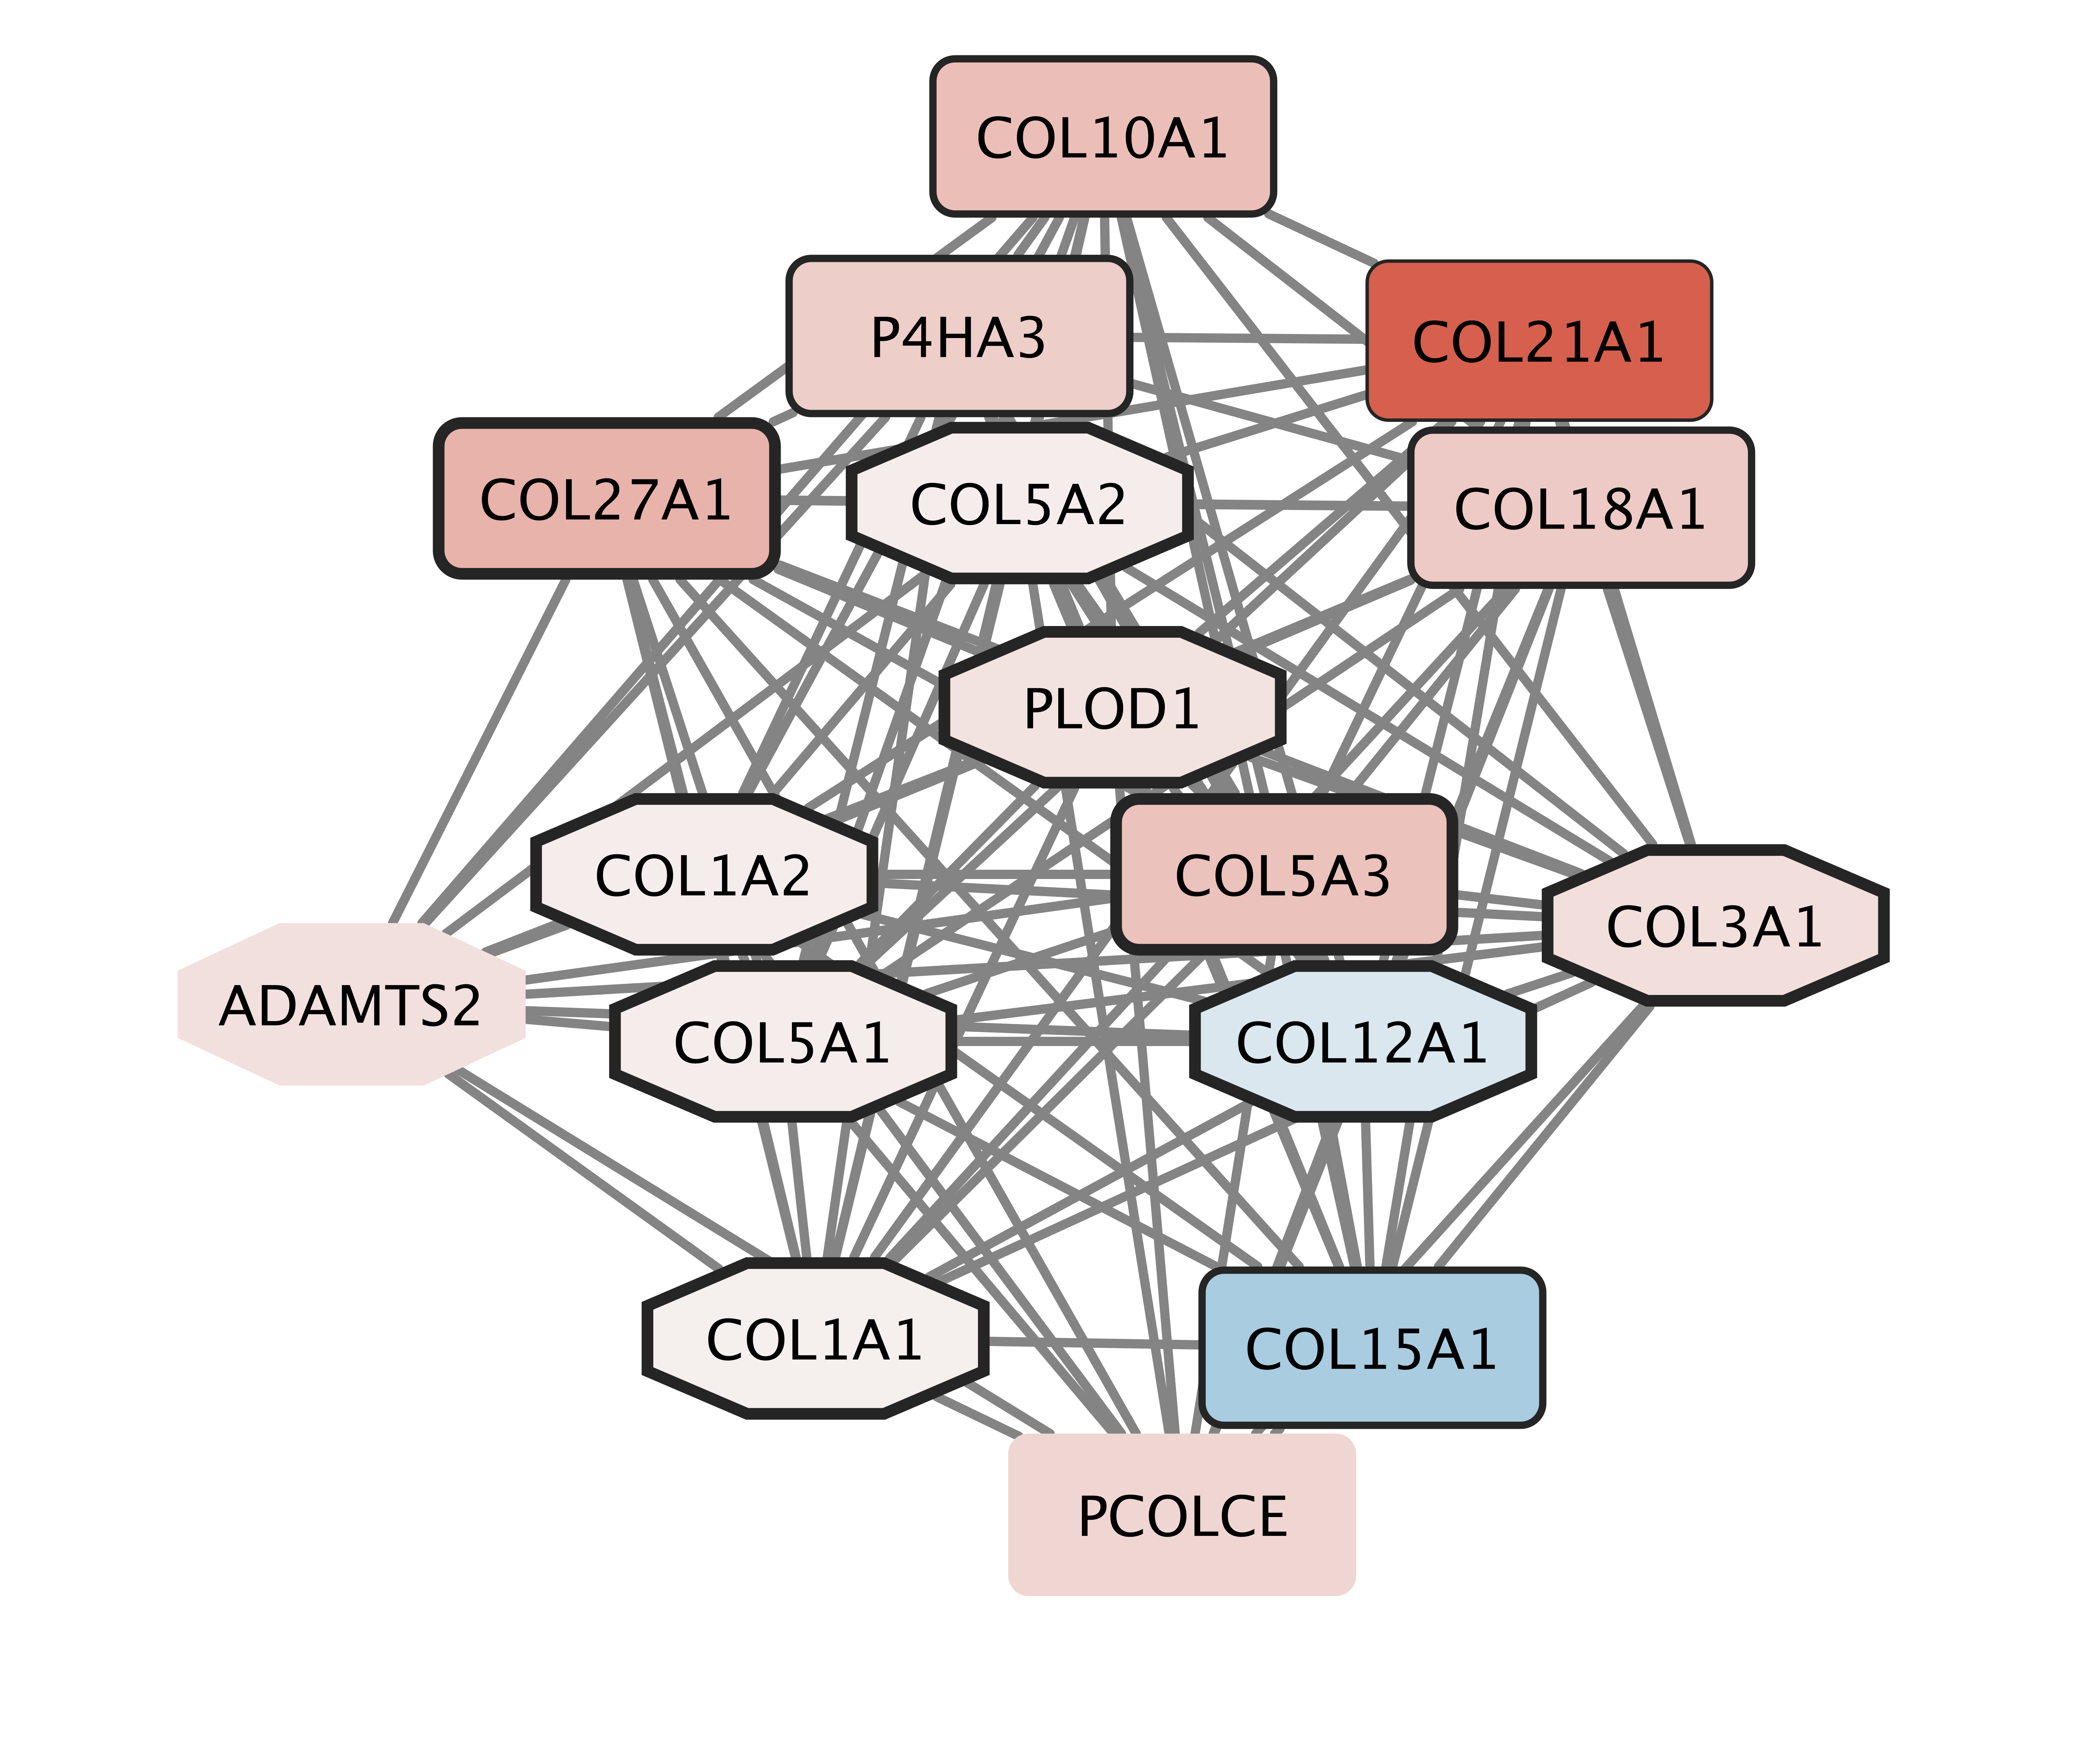
\includegraphics[width=0.7\textwidth]{fig/MCODE-cluster3.png}
	\caption[MCODE cluster 3]{\centering The MCODE cluster contains many genes known to cause other types of EDS. [TODO: add legend for shape, border and colour]}
	\label{fig:mcode3}
\end{figure}

GO-Enrichment testing overrepresentation of molecular functions of the cluster returns extracellular matrix in two terms.
\begin{itemize}
	\item quite interesting to see genes closely related to other eds genes, COL21A1 is also strongly upregulated ($\text{log2FoldChange} > 2$)
	\item regarding the enrichment of this cluster: not surprising to see the extracellular matrix in two GO-Terms when testing for over-representation of molecular functions
	\item this was found by simila research as well \cite{Ritelli2022} [Todo: there was other ressearch, find]
	\item first go term: GO:0005201 - The action of a molecule that contributes to the structural integrity of the extracellular matrix. overall 13 of the 16 genes in this GO-Term, 6 are known eds genes, the other six differentially expressed (COL10A1, COL15A1, PCOLCE, COL5A3, COL18A1, COL21A1, COL27A1)
	\item second go term: GO:0030020 - A constituent of the extracellular matrix that enables the matrix to resist longitudinal stress, and is a subtype of the first. Same EDS genes and same genes as in the first term, except PCOLCE, PCOLE is also the only downregulated gene [TODO: interprete]
	\item affection of ECM shown in earlier research as well, particularly disorganization of collagen and fibronectin in hEDS and two other EDS types \cite{Chiarelli2018}
	\item thus look how central genes lay in the enrichment term and how strong is their differential expression
	\item COL27A1 fibrillar collagen gene, protein codingf gene
	\item COL5A3 alpha chain for fibrillar collagens
	\item COL21A1 alpha chain of type XXI collagen, maintains integrity of ECM, therefore really interesting, paralog to COL5A1 (other EDS gene) [TODO: cite https://www.ncbi.nlm.nih.gov/gene/81578\#summary]
\end{itemize}

\begin{itemize}
	\item mcode cluster 2: 	GO:0030527 - structural constituent of chromatin enriched, downregulated genes involved in processes related to chromatin in vEDS \cite{Chiarelli2018}
\end{itemize}

\subsubsection{Community Clustering}

\begin{itemize}
	\item 6 clusters with more than 15 nodes
	\item 3 very small loosely connected clusters (18 nodes \& 17 connections, 29 nodes \& 32 connections, 29 nodes \& 29 connections), two medium-sized highly interconnected (76 nodes \& 1000 connections and 105 nodes \& 2330 connections) and one very large cluster (363 nodes \& 1661 connections)
	\item especially medium-sized clusters highly interconnected
	\item both medium-sized clusters mostly upregulated $\rightarrow$ interesting!
	\item smallest cluster with 18 nodes to small for meaningful enrichment analysis regarding processes
\end{itemize}

\paragraph{Largest Community Cluster}

\begin{itemize}
  \item mix of up-regulated and down-regulated genes, contains all 21 genes known to cause other EDS types
\end{itemize}

